\documentclass[]{llncs}

\usepackage{vmargin}
\usepackage{caption} 
\captionsetup[table]{skip=8pt}
\usepackage{hyperref}
\usepackage[pdftex]{color,graphicx}
\usepackage{amssymb}
%\usepackage{amsmath} % assumes amsmath package installed
\usepackage{fancyvrb,fancyhdr}
\usepackage{listings}
\usepackage[spanish, activeacute]{babel}
\usepackage[utf8]{inputenc}
\usepackage{listingsutf8}
\pagenumbering{arabic}
\usepackage{lastpage}

\pagestyle{plain}

%*********************** FORMATO DE LISTADOS **************************
\lstset{
  basicstyle=\tiny,
  keywordstyle=\bfseries,
  % underlined bold black keywords
  identifierstyle=, % nothing happens
%  commentstyle=\color{white}, % white comments
  stringstyle=\ttfamily, % typewriter type for strings
  showstringspaces=false,
  frame=single,
  language=Java,
  numbers=left,
  numberstyle=\tiny,
  stepnumber=2,
  numbersep=5pt,
  inputencoding=utf8
}

%******************** PARRAFOS ****************************************
\setlength{\parindent}{0pt}
\setlength{\parskip}{0.8em}

\author{César Antonio Enrique Ramírez}
\title{Controlador de aparcamiento usando lógica difusa}
\institute{Universidad de Huelva}

\begin{document}
\maketitle
\begin{abstract}
  En el presente documento se expone el desarrollo de varios módulos
  escritos en Haskell con el objetivo de utilizarlos para definir
  sistemas basados en lógica difusa y describir un controlador difuso
  de aparcamiento en batería con ellos. El desarrollo de este trabajo
  está basado en \cite{kosko1992}
\end{abstract}
\section{Introducción}
La lógica difusa es un tipo de lógica en el que las proposiciones no
son verdaderas o falsas, sino que tienen un \emph{grado de verdad} que se
representa mediante un número real comprendido entre 0 y 1. El valor 0
indica que la proposición es totalmente falsa. El valor 1 indica que
la proposición es totalmente verdadera. Los valores intermedios
indican que la proposición debe considerarse verdadera en cierto
grado.

Los diferentes conceptos usados en lógica difusa se representan
mediante fuciones de pertenencia. Estas fuciones pueden tener muchas
formas, pero generalmete para describir conceptos relacionados con
variables continuas se utilizan fuciones de pertenencia con forma de
triángulo, trapezoide, rampa, campana, sigmoide, etc.

Una proposición difusa básica expresa la relación entre el valor de
una cierta variable y un concepto. Por ejemplo, \emph{la temperatura es
alta} es una proposición difusa que relaciona la variable \emph{temperatura}
con el concepto \emph{alta}. Al evaluar la proposición aplicando el
valor de la variable a la función de pertenencia, obtenemos un valor
entre 0 y 1 que representa el \emph{grado de activación} de la proposición.

Las proposiciones difusas se componen por medio de operaciones AND y
OR. Estas operaciones representan los operadores lógicos AND y OR,
pero deben ser funciones definidas sobre valores reales entre 0 y 1
para poder aplicarlas a valores difusos. Las funciones que cumplen
este requisito se llaman T-normas y S-normas. Las T-normas más
utilizadas para representar la operación AND and son el mínimo o el
producto (en esta implementación usaremos el producto). Para
representar la operación OR se utilizan el máximo o la suma acotada
entre otras (en nuestro caso usaremos la suma algebraica).

Una regla difusa es una contrucción del tipo \emph{if ... then ...}
donde el antecedente de la regla es una proposición difusa.

Una base de reglas es un conjunto de reglas en las que las variables
de entrada del sistema se usan en el antecedente y las variables de
salida se usan en los consecuentes. Mediante un método de
``defuzzificación'' se obtienen las variables de salida a partir del
grado de activación de las reglas y su consecuente.
\section{Implementación}
Para la implementación de este sistema difuso se ha dividido la
funcionalidad en tres módulos:

\begin{itemize}
\item El módulo \emph{Fuzzy.hs} contiene la definición de los tipos de
  datos necesarios para la implementación del resto de módulos.
\item El módulo \emph{FuzzyLib.hs} contiene la definición de
  funciones de pertenencia, así como de T-normas, S-normas y funciones
  de defuzzificacion.
\item El módulo \emph{FuzzyParking.hs} contiene la definición concreta
  del sistema difuso para el problema del aparcamiento en batería.
\end{itemize}

En esta memoria no entraremos en detalle con cada uno de ellos por ser
relativamente sencillos además de estar debidamente documentados, por
lo que en vez de eso, nos detendremos a analizar detalladamente
algunas partes clave del funcionamiento del sistema.

El primer trozo de código que analizaremos corresponde a la definición
de una fución de pertenencia. Para ilustrar la técnica que hemos usado
vamos a emplear la fución de pertenencia con forma de triángulo, pero
el concepto se aplica igual con el resto.

\begin{figure}
\begin{lstlisting}
triangle :: (Float, Float, Float) -> MemFunc
triangle (a,b,c) f
  | f > a && f <= b = (f-a) / (b-a)
  | f > b && f < c  = 1 - (f-b) / (c-b)
  | otherwise       = 0
\end{lstlisting}
\caption{Función de pertenencia en forma de triángulo}
\label{code:codigo1}
\end{figure}

Como podemos ver en la figura \ref{code:codigo1}, la función
\emph{triangle} es de tipo \emph{(Float, Float, Float) -> MemFunc}, lo
que quiere decir que toma como parámetro una tupla con tres valores
reales y devuelve un valor de tipo \emph{MemFunc}, que está definido
en el módulo \emph{Fuzzy.hs}.

\begin{figure}
\begin{lstlisting}
type memFunc = (Float -> Fuzzy)
\end{lstlisting}
\label{code:codigo2}
\end{figure}

Por lo tanto, la función \emph{triangle} recibe como parámetro una
tupla y devuelve una fución, la cual toma como parámetro un valor real
y de vuelve un \emph{Fuzzy} (que no es más que un valor real entre 0 y
1).

El tipo de la función \emph{triangle} se podría reescribir como
\begin{figure}
\begin{lstlisting}
triangle :: (Float, Float, Float) -> Float -> Fuzzy
\end{lstlisting}
\label{code:codigo3}
\end{figure}
y sería totalmente válido, sin embargo utilizamos el tipo
\emph{MemFunc} para hacer énfasis en que lo que devuelve no es sólo el
\emph{Fuzzy} que aparece al final de la definición del tipo, sino una
función de tipo \emph{Float -\textgreater Fuzzy}. Esto es así gracias a la
aplicación parcial de funciones. De hecho, la definición de la función
tiene cuatro parámetros de entrada, pero cuando la llamamos en el
resto del código sólo le pasamos tres. De esta forma, podemos definir
funciones de pertenencia parametrizadas sin necesidad de progrmarlas a
mano todas.

Los tres parámetros en la tupla que recibe la fución \emph{triangle}
corresponden a los tres vértices del triángulo descritos en una
dimensión, teniendo en cuenta que la altura del triángulo es siempre 1.

El siguiente trozo de código corresponde a una función de
defuzzificaicón. En concreto a la función \emph{wightedFuzzyMean}.

\begin{figure}
\begin{lstlisting}
weightedFuzzyMean :: Defuzmethod
weightedFuzzy x = foldr (\(c,d,a) acc -> acc + (a*d*c)) 0 x /
  (foldr (\(_,d,a) acc -> acc + (a*d)) 0 x)
\end{lstlisting}
\caption{Función de defuzzificación usando la media difusa ponderada
  por la base}
\label{code:codigo4}
\end{figure}

En este caso, vemos una declaración de tipo \emph{Defuzmethod}, que no
es más que \emph{[(Float, Float, Float)] -\textgreater Float}. Esta
función calcula la media de los centros de los consecuentes de cada
regla, ponderados por el producto entre el grado de activación de la
regla y la base o el área del consecuente. La expresión \ref{exp:expresion1}
corresponde a su funcionamiento.

\begin{equation}
y = \frac{\sum_{r} \alpha_{r} \cdot d_{r} \cdot c_{r}}{\sum_{r}
  \alpha_{r} \cdot d_{r}}
\label{exp:expresion1}
\end{equation}

Los tres parámetros que recibe la función \emph{weightedFuzzyMean} en
cada tupla de la lista corresponden a el centro de la función de
pertenencia del consecuente, la base de la misma, y el grado de
activación de la regla en la que aparece dicho conseguente.

La siguiente función que vamos a analizar es la función que realiza la
inferencia, \emph{fuzzyParking}.

\begin{figure}
\begin{lstlisting}
fuzzyParking :: Inference -- [Float] -> Float
fuzzyParking sys (x:a:_) = (defuzmethod sys) $ zip3 centros base alphaList
  where alphaList = map (evalTerm (tnorma sys) (snorma sys) . tmap f . getTerm) $ reglas sys
        params = unzip . map (getParams . getConseq) $ (reglas sys)
        centros = fst params
        base = snd params
        f var = case var of
          "X"      -> x
          "Angulo" -> a
\end{lstlisting}
\caption{Función que realiza la inferencia del sistema de aparcamiento
  en batería}
\label{code:codigo5}
\end{figure}

Esta función toma como parámetros un sistema difuso y una lista de
parámetros de entrada para el sistema. En este caso concreto nuestro
sistema sólo utiliza dos entradas. Para calcular el resultado a
devolver, la función tendrá que aplicar las entradas a las reglas del
sistema y calcular el valor de salida usando el método de
defuzzificación del sistema, como podemos ver en la línea 2 de la
figura \ref{code:codigo5}.

Para calcular el grado de activación de cada regla se mapea la función
\emph{evalTerm} sobre todas las reglas. Podemos ver esta función en la
figura \ref{code:codigo6}.

\begin{figure}
\begin{lstlisting}
evalTerm :: Tnorm -> Snorm -> Term -> Fuzzy
evalTerm and or (t1 :&& t2)          = (evalTerm and or t1) `and` (evalTerm and or t2)
evalTerm and or (t1 :|| t2)          = (evalTerm and or t1) `or`  (evalTerm and or t2)
evalTerm and or ((Val x) := memFunc) = memFunc x
evalTerm _   _   _                   = 0
\end{lstlisting}
\caption{Función que evalúa un término difuso, calculando así el grado de activación}
\label{code:codigo6}
\end{figure}

Pero primero se necesita sustituir cada variable en las reglas por su
correspondiente valor de entrada. Para eso usamos la función
\emph{tmap}, que aunque no es exactamente igual, recuerda a
\emph{fmap} en su funcionamiento, pero debido a sus restricciones no
podemos declarar una instancia de \emph{Functor}. Podemos ver esta
función en la figura \ref{code:codigo7}.

\begin{figure}
\begin{lstlisting}
tmap :: (String -> Float) -> Term -> Term
tmap f (l :&& r) = (tmap f l) :&& (tmap f r)
tmap f (l :|| r) = (tmap f l) :|| (tmap f r)
tmap f ((Var x) := mem) = (Val $ f x) := mem
\end{lstlisting}
\caption{Función que aplica una función de String a Float a la
  estuctura de un Term}
\label{code:codigo7}
\end{figure}

Lo siguiente será echar un vistazo a cómo definimos el sistema difuso,
y para eso vamos a ver cómo definimos una regla.

Abusando un poco del sistema de tipos de haskell, hemos ideado una
forma de construir los tipos que nos permite describir las reglas con
una sintaxis no demasiado incómoda, siendo bastante fáciles de leer en
código directamente. Primero veamos el tipo Term, tal y como aparece
en la figura \ref{code:codigo8}. Está formado por tres constructores,
pero no son contructores normales, son \emph{infijos}. Podemos
observar también que la definición es recursiva, y que el caso base es
en el que \emph{Term} está definido como una asignación de una función
de pertenencia a una variable.

\begin{figure}
\begin{lstlisting}
data Term = (Term) :&& (Term) | (Term) :|| (Term) | (Var) := (MemFunc)
\end{lstlisting}
\caption{Tipo de dato que representa una proposición difusa.}
\label{code:codigo8}
\end{figure}

Examinemos a continuación el tipo Rule. Podemos verlo en la figura
\ref{code:codigo9}. Su constructor \emph{IF} representa
convenientemente el comienzo de una expresión lógica, a continuación
recibe un \emph{Term} y por último un \emph{Conseq}. La estructura es
muy clara: \emph{IF regla-difusa consecuente}. También podemos ver en
la figura \ref{code:codigo10} que el constructor del tipo
\emph{Conseq} también está convenientemente nombrado como \emph{THEN},
por lo que nos queda una estructura del tipo:

\begin{equation}
IF ((variable := metodo) :\&\& (variable2 := metodo2) :\&\& ...) \$
THEN consecuente 
\end{equation}

Es importante fijarnos en el símbolo \$ que hay entre la parte del
antecedente y \emph{THEN}. En vez de eso podemos usar paréntesis
rodeando a todo el consecuente.

En la figura \ref{code:codigo11} podemos ver código en el que se 
definen algunas reglas.

\begin{figure}
\begin{lstlisting}
data Rule = IF Term Conseq
\end{lstlisting}
\caption{Tipo de dato que representa una regla del sistema difuso.}
\label{code:codigo9}
\end{figure}

\begin{figure}
\begin{lstlisting}
data Conseq = THEN Var (Float, Float)
\end{lstlisting}
\caption{Tipo de dato que representa el consecuente de una regla.}
\label{code:codigo10}
\end{figure}

\begin{figure}
\begin{lstlisting}
reglas = [
IF ((Var "X" := lE) :&& (Var "Angulo" := rB)) $ THEN (Var "volante") (sera3 ps),
IF ((Var "X" := lE) :&& (Var "Angulo" := rU)) $ THEN (Var "volante") (sera3 ns),
IF ((Var "X" := lE) :&& (Var "Angulo" := rV)) $ THEN (Var "volante") (sera3 nm),
IF ((Var "X" := lE) :&& (Var "Angulo" := vE)) $ THEN (Var "volante") (sera3 nm),
...
]
\end{lstlisting}
\caption{Reglas del sistema difuso escritas con una sintaxis facil de leer.}
\label{code:codigo11}
\end{figure}

Por último, tenemos la función \emph{main}, la cual podemos ver en la
figura \ref{code:codigo12}, que calcula la
salida del sistema difuso para todos los posibles valores del ángulo y
la distancia. Con estos valores podremos representar gráficamente al
sistema.

\begin{figure}
\begin{lstlisting}
main :: IO ()
main = putStrLn $ (unlines . map (unwords . map (show))) vs
  where vs = [[a,x,fuzzyParking system [x,a]] | x <- [-50,-45..50], a <- [-180,-170..180]]
\end{lstlisting}
\caption{Función main, que calcula la salida del sistema difuso para
  todos los posibles valores de entrada.}
\label{code:codigo12}
\end{figure}
\section{Grafica}

Si representamos los datos obtenidos de la ejecución del programa
vemos como la gráfica representa una superficie con varios
niveles. Dichos niveles corresponden con las reglas que hemos definido
para el sistema, basándonos en las definidas en \cite{kosko1992}.

\begin{figure}
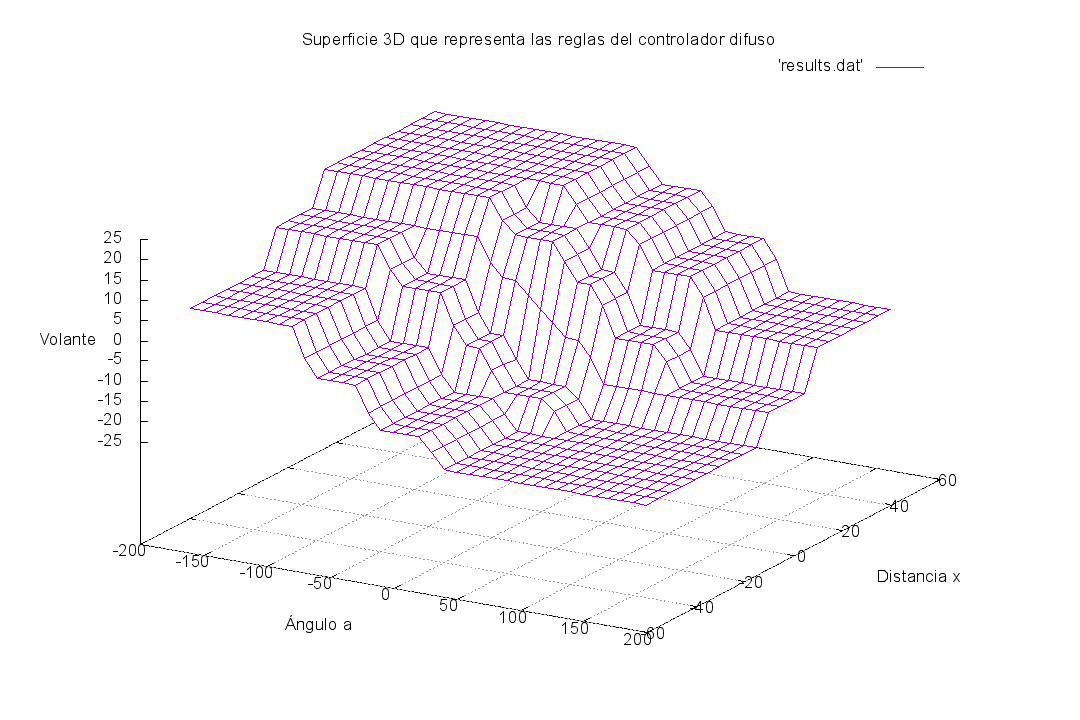
\includegraphics[width=\textwidth,height=\textheight,keepaspectratio]{superficie-resultado.png}
\caption{Representación gráfica de la salida del sistema para todos
  los valores posibles.}
\label{img:grafica2}
\end{figure}

\section{Pruebas}
Las puebas se han diseñado usando el framework \emph{HUnit}. Podemos
ver los diferentes casos de prueba que se han diseñado en la figura \ref{code:codigo13}.

\begin{figure}
\begin{lstlisting}
tests = test [ 
"test-triangle-move1" ~: (triangle (5,6,7)) 5.3 ~=? ((triangle (-5,-4,-3)) . flip (-) 10) 5.3,
"test-triangle-move2" ~: (triangle (5,6,7)) 6.3 ~=? ((triangle (-5,-4,-3)) . flip (-) 10) 6.3,
"test-triangle-move3" ~: (triangle (5,8,9.5)) 6 ~=? ((triangle (-5,-2,-0.5)) . flip (-) 10) 6,

"test-trapezoid-move1" ~: (trapezoid (5,8,9.5, 10)) 6 ~=? ((trapezoid (-5,-2,-0.5, 0)) . flip (-) 10) 6,
"test-trapezoid-move2" ~: (trapezoid (5,8,9.5, 10)) 9 ~=? ((trapezoid (-5,-2,-0.5, 0)) . flip (-) 10) 9,
"test-trapezoid-move3" ~: 
  (trapezoid (5,8,9.5, 10)) 9.7 ~=? ((trapezoid (-5,-2,-0.5, 0)) . flip (-) 10) 9.7,

"test-sramp-move1" ~: (sramp (5,8)) 9 ~=? ((sramp (-5,-2)) . flip (-) 10) 9,
"test-sramp-move2" ~: (sramp (5,8)) 7 ~=? ((sramp (-5,-2)) . flip (-) 10) 7,

"test-zramp-move1" ~: (zramp (5,8)) 4 ~=? ((zramp (-5,-2)) . flip (-) 10) 4,
"test-zramp-move2" ~: (zramp (5,8)) 7 ~=? ((zramp (-5,-2)) . flip (-) 10) 7,

"test-trapezoid1" ~: (trapezoid (5,8,9.5, 10)) 4 ~=? 0,
"test-trapezoid21" ~: (trapezoid (5,8,9.5, 10)) 6 > 0 ~? "",
"test-trapezoid22" ~: (trapezoid (5,8,9.5, 10)) 6 < 1 ~? "",
"test-trapezoid3" ~: (trapezoid (5,8,9.5, 10)) 9 ~=? 1,

"test-sramp-zramp" ~: (sramp (5,8)) 7 ~=? (1 - ((zramp (5,8))  7)),

"test-tnormMin" ~: tnormMin 0.5 0.8 ~=? 0.5,
"test-tnormProd" ~: tnormProd 0.5 0.8 ~=? 0.4,
"test-snormMax" ~: snormMax 0.5 0.8 ~=? 0.8,
"test-snormSum" ~: snormSum 0.5 0.8 ~=? 0.9,

"test-2fuzzyMean" ~: 
   fuzzyMean [(10, 20, 0.5), (30, 20, 0.1)] ~=? weightedFuzzyMean [(10, 20, 0.5), (30, 20, 0.1)]
             ]
\end{lstlisting}
\caption{casos de prueba}
\label{code:codigo13}
\end{figure}
\section{Conclusión}
Para concluir, podemos decir que el desarrollo de un sistema difuso se
adecua mucho a las caracteríasticas y funcionalidades que proporciona
Haskell tanto por su sintaxis como por usar el paradigma de
programación funcional. El sistema no ha sido complicado de
desarrollar pero si muy reconfortante cuando ves los resultados. Como
cosas a mejorar, se podría hacer una parser para obtener el systema
difuso desde una especificación en un fichecho externo, y desarrollar
funcionalidad que permita fácilmente procesar sistemas con más de una
variable de salida, ya que en lo que a esta implementación respecta,
por parte de las librerías sí está soportado, pero lo que es el
sistema difuso para el controlador de aparcamiento en batería, como
solo tiene una variable de salida no se ha implentado el manejo de
reglas con diferentes variables en el consecuente.
\section{Código}
El código de este trabajo se puede descargar desde el repositorio
\url{git@github.com:caenrique/fuzzyParking.git}, o revisarlo online
desde \url{https://github.com/caenrique/fuzzyParking}.

\bibliographystyle{acm}
\bibliography{bibliografia}


\end{document}
